In  diesem  Versuch kommen  verschiedene  Bereiche  aus der  Physik  zusammen,
prim\"ar Fluid-Dynamik und Optik. Entsprechend ergibt sich auch die Gliederung
dieses Kapitels.

% ---------------------------------------------------------------------------- %
\subsection{Messprinzip}
\label{subsec:messprinzip}
% ---------------------------------------------------------------------------- %

Das Verfahren nutzt den optischen  Dopplereffekt, um die Geschwindigkeit eines
Teilchens in einem  Fluid zu detektieren. Trifft ein  Lichtstrahl der Frequenz
$f$ auf  ein bewegtes Objekt,  unterschheidet sich die vom  Objekt detektierte
Frequenz $f_1$ ein wenig von der vom Sender emittierten Frequenz $f_0$.

\begin{equation}
    \label{eq:doppler}
    f_1 = f_0 \cdot \left( 1 - \frac{\vec{e} \cdot \vec{v}}{c} \right)
        = f_0 \cdot \left( 1 + \frac{v}{c} \cdot \cos{\vartheta_1} \right)
\end{equation}

Wobei $c$  die Lichtgeschwindigkeit, $\vec{e}$ ein  Einheitsvektor in Richtung
des  Lichtstrahls  und  $\vec{v}$   der  Geschwindigkeitsvektor  des  bewegten
Objektes ist. Wird der Lichtstrahl am bewegten Objekt gestreut und anschliessend
von einem Empf\"anger detektiert, ergibt sich f\"ur diesen die Frequenz $f_2$:

\begin{equation}
    \label{eq:doppler:gestreut}
    f_2
        = f_1 \cdot \left( 1 + \frac{\vec{a} \cdot \vec{v}}{c} \right)
        = f_0 \cdot \left( 1 - \frac{\vec{e} \cdot \vec{v}}{c} \right)
              \cdot \left( 1 + \frac{\vec{a} \cdot \vec{v}}{c} \right)
        \approx
        f_0 \cdot
        \left(
            1
            -
            \frac{\vec{a} \cdot \vec{v}}{c}
            +
            \frac{\vec{e} \cdot \vec{v}}{c}
        \right)
\end{equation}

$\vec{a}$   ist    dabei   ein   Einheitsvektor   in    Ausfallsrichtung   des
gestreuten   Strahls. Die   Konfiguration   ist   schematisch   in   Abbildung
\ref{fig:dopplereffekt} dargestellt.

\begin{figure}[h!t]
    \centering
    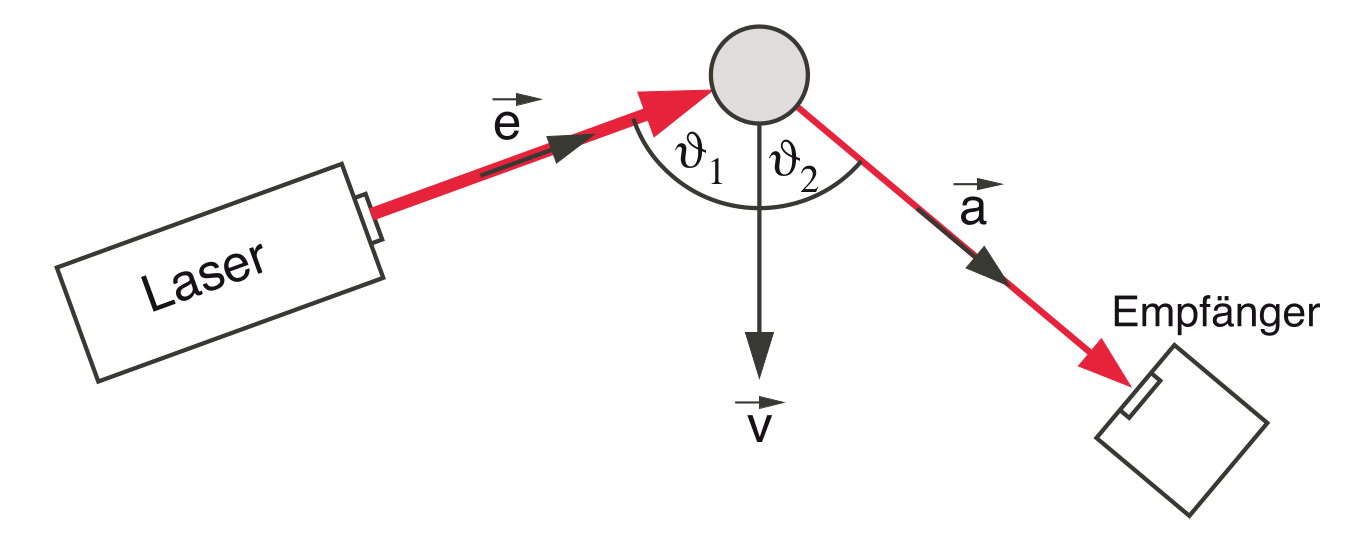
\includegraphics[width=0.67\textwidth]{images/doppler-effekt.png}
    \caption{%
        Dopplereffekt   mit  station\"arem   Sender,   bewegtem  Streuer   und
        station\"arem Detektor. \quelleVA
    }
    \label{fig:dopplereffekt}
\end{figure}

Da  bei  technischen  Geschwindigkeiten das  Verh\"altnis  $\frac{v}{c}$  sehr
klein   ist,  ergeben   sich  unter   solchen  Umst\"anden   lediglich  minime
Unterschide  in   den  Frequenzen  $f_4$,  $f_1$   und  $f_2$. Eine  pr\"azise
Messung  der  Frequenzunterschiede  ist  somit enorm  schwierig,  weshalb  man
sich  eines Zwei-Stral-Verfahrens  bedient. Da die  beiden Teilstrahlen  dabei
in  unterschiedlichen  Winkeln  $\vartheta_1$  (vgl. Formel  \ref{eq:doppler})
auf   das   streuende   Teilchen  treffen,   erfahren   sie   unterschiedliche
Doppler-Verschiebungen ihrer Frequenzen.

\"Uberlagert man  nun die beiden  Teilstrahlen in einem Detektor,  ergibt sich
eine  Schwebung, deren  Frequenz bedeutend  tiefer  als $f_0$  ist, und  somit
verh\"altnism\"assig gut detektiert werden kann.

Eine     h\"aufig     verwendete     Konfiguration    ist     in     Abbildung
\ref{fig:zweistrahl-anordnung} zu sehen.

\begin{figure}[h!t]
    \centering
    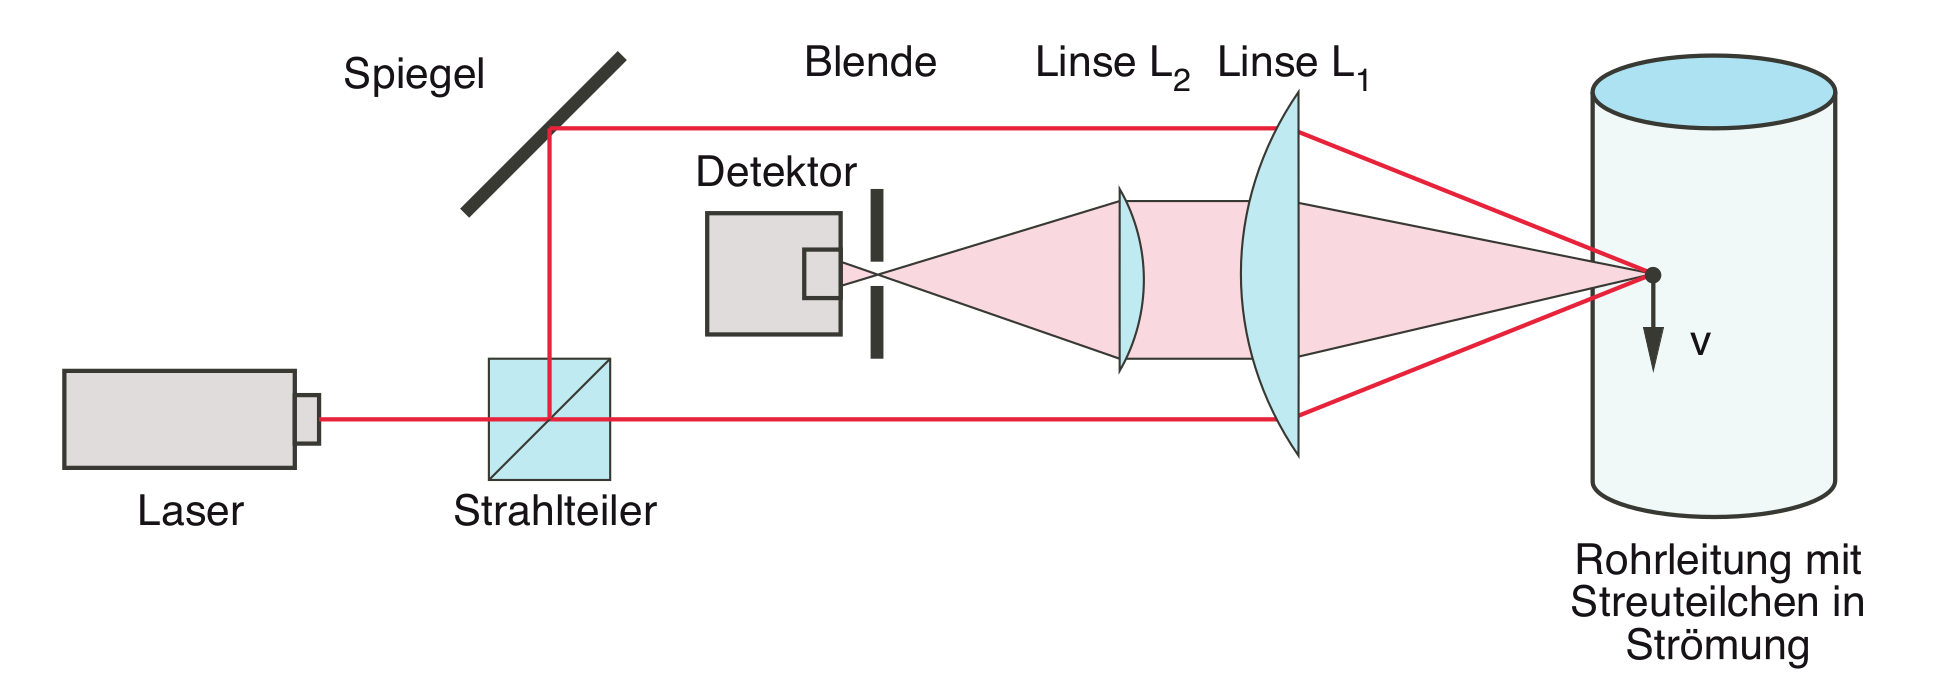
\includegraphics[width=0.67\textwidth]{images/zweistrahl-anordnung.png}
    \caption{%
        Zwei-Srahl-Anordnung. \quelleVA
    }
    \label{fig:zweistrahl-anordnung}
\end{figure}

Ein Strahlteiler teilt  den Laserstrahl auf zwei Strahlen auf  und ein Spiegel
sorgt daf\"ur, dass zwei parallele  Strahlen entstehen, die anschliessen durch
eine Linse $L_1$ mit Brennweite $f_1$ wieder zusammengef\"uhrt werden. Fliesst
ein Streuteilchen durch diesen Schnittpunkt, ergeben sich f\"ur die beiden Teilstrahlen
zwei unterschiedliche Frequenzen aufgrund des Dopplereffekts:

\begin{align}
    \label{eq:splitFreqs1}
        f_1 &= f_0 \cdot
            \left(
                1 + \frac{v}{c} \cdot \cos\left( \SI{90}{\degree} + \frac{\varphi}{2} \right)
            \right)
            =
            f_0 \cdot
            \left(
                1 - \frac{v}{c} \cdot \sin\left(\frac{\varphi}{2}\right)
            \right)
            \\
        \label{eq:splitFreqs2}
        f_2 &= f_0 \cdot
            \left(
                1 + \frac{v}{c} \cdot \cos\left( \SI{90}{\degree} - \frac{\varphi}{2} \right)
            \right)
            =
            f_0 \cdot
            \left(
                1 + \frac{v}{c} \cdot \sin\left(\frac{\varphi}{2}\right)
            \right)
            \\
        \label{eq:splitFreqsDelta}
        \Delta f &= f_2 - f_1 = f_0 \cdot \frac{2 \cdot v}{c} \cdot \sin\left( \frac{\varphi}{2}\right)
\end{align}

Die beiden  Wellenz\"uge werden  anschliessend in einem  einzelnen Empf\"anger
zusammengef\"uhrt. Die durch diese \"Uberlagerung erzeugte Schwebung errechnet
sich  nach  einigen  trigonometrischen  Umformungen zu  (beachte,  dass  beide
Signale die gleiche Amplitude haben, was die Sache etwas vereinfacht):

\begin{equation}
    \label{eq:schwebung}
    S(t) = A \cdot \cos(\omega_1 \cdot t) + A \cdot \cos(\omega_2 \cdot t)
         = 2 A \cdot
             \cos\left(
                 \frac{\omega_1 + \omega_2}{2} \cdot t
             \right)
             \cdot
             \cos\left(
                 \frac{\omega_1 - \omega_2}{2} \cdot t
             \right)
\end{equation}

% ---------------------------------------------------------------------------- %
\clearpage
\subsection{Grundlagen aus der Fluid-Dynamik}
\label{subsec:fluiddynamik}
% ---------------------------------------------------------------------------- %

\subsubsection{Vorbereitung auf Messaufgaben}

3.1 -- Zusammenhang zwischen maximaler und durchschnittlicher Str\"omungsgeschwindigkeit im laminaren Fall

\textbf{fix: avg over flaeche}
\begin{equation}
    \label{eq:laminar:v_max:v_avg}
    \frac{v(r)}{v_{max}} = \frac{1}{v_{max} \cdot R} \cdot \int_0^R\!v(r) \, \mathrm{d}r
    = \frac{1}{R} \cdot \int_0^R \! 1 - \frac{r^2}{R^2} \, \mathrm{d}r
    = \frac{1}{2}
\end{equation}

3.2 -- Zusammenhang zwischen maximaler und durchschnittlicher Str\"omungsgeschwindigkeit im turbulenten Fall:

\begin{align}
    \label{eq:turbulent:v_max:v_avg}
    v(r) &= v_{max} \cdot \left( 1 - \frac{r}{R} \right) ^ \frac{1}{k}
    \\
    v_m &= \frac{1}{\pi \cdot R^2} \cdot \int_0^R \! v(r) \cdot 2 \cdot \pi \cdot r \, \mathrm{d}r
    \\
    \frac{v_m}{v_{max}} &= \frac{2}{R^2} \cdot \int_0^R \! \left(1 - \frac{r}{R} \right) ^ \frac{1}{k} \cdot r \, \mathrm{d}r = \frac{2 \cdot k^2}{(k + 1) \cdot (2k + 1)}
\end{align}

3.3 -- Vergleich von laminarem und turbulentem Str\"omungsprofil

\begin{figure}[h!t]
    \centering
    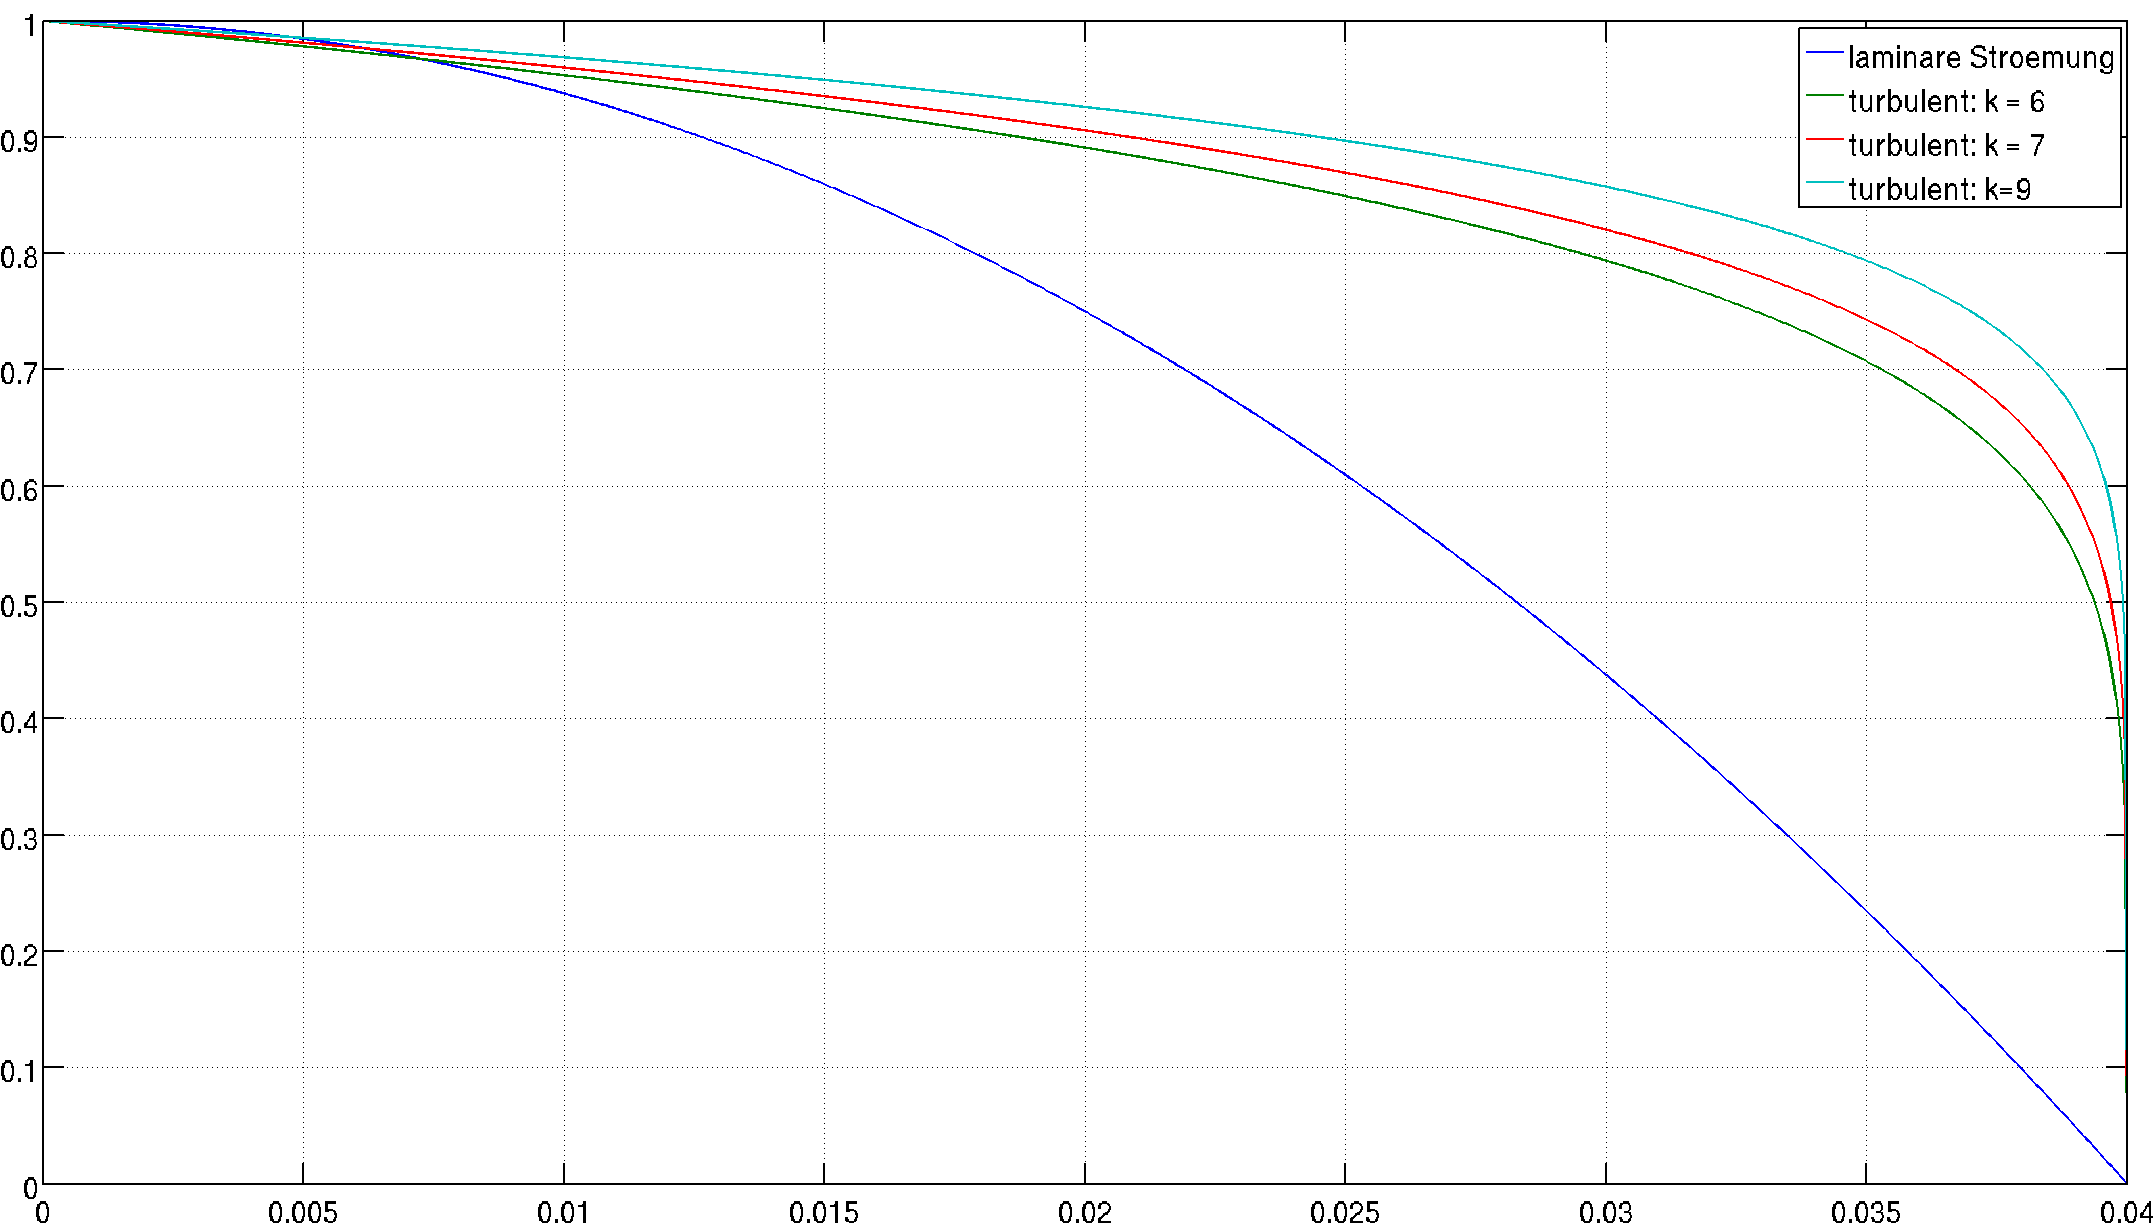
\includegraphics[width=\textwidth]{images/laminar-vs-turbulent.png}
    \caption{%
        Laminares vs. turbulente Str\"omungsprofile
    }
    \label{fig:dopplereffekt}
\end{figure}


\clearpage
3.4 -- Volumenstrom und Rohrradius bei gleichem Druckgef\"alle

(via Sympy)


\begin{equation}
    \label{eq:q:r}
    Q = \frac{\pi \cdot R^4 \cdot \Delta \, p}{8 \cdot \eta \cdot l}
\end{equation}


3.5 -- Reynoldszahlen

\begin{equation}
    \label{eq:reynolds1}
    Re = \frac{\rho \cdot v_m \cdot L}{\eta}
\end{equation}

\begin{align}
    \dot{V}_{min} = \SI{0.5}{\liter\per\minute} = \SI{8.3e-6}{\cubic\meter\per\second}
    \\
    \dot{V}_{max} = \SI{7.5}{\liter\per\minute} = \SI{125e-6}{\cubic\meter\per\second}
    \\
    A = \pi \cdot R^2 = \SI{0.00126}{\meter\squared}
    \\
    v_{m,min} = \frac{\dot{V}_{min}}{A} = \SI{0.0066}{\meter\per\second}
    \\
    v_{m,max} = \frac{\dot{V}_{max}}{A} = \SI{0.099}{\meter\per\second}
    \\
    Re_{min} = \frac{\rho \cdot v_{m,min} \cdot 2R}{\eta} = 264
    \\
    Re_{max} = \frac{\rho \cdot v_{m,max} \cdot 2R}{\eta} = 3960
    \\
    %f_{Signal} = \frac{f_2 - f_1}{2} = \frac{f_0}{2} \cdot \left( \left(1 + \frac{v}{c}\sin\left(\frac{\varphi}{2}\right)\right) - \left(1 - \frac{v}{c}\sin\left(\frac{\varphi}{2}\right)\right)\right)
    %= f_0 \cdot \frac{v}{c} \sin\left(\frac{\varphi}{2}\right)
    \Delta\,f = \frac{2\sin\left(\frac{\varphi}{2}\right) \cdot v}{\lambda} = \left\{ \SI{13.11}{\hertz}, \SI{197.5}{\hertz} \right\} \mathrm{~f\"ur \varphi = \SI{30}{\degree}}
\end{align}
